\documentclass{standalone}
\usepackage{tikz}
\begin{document}
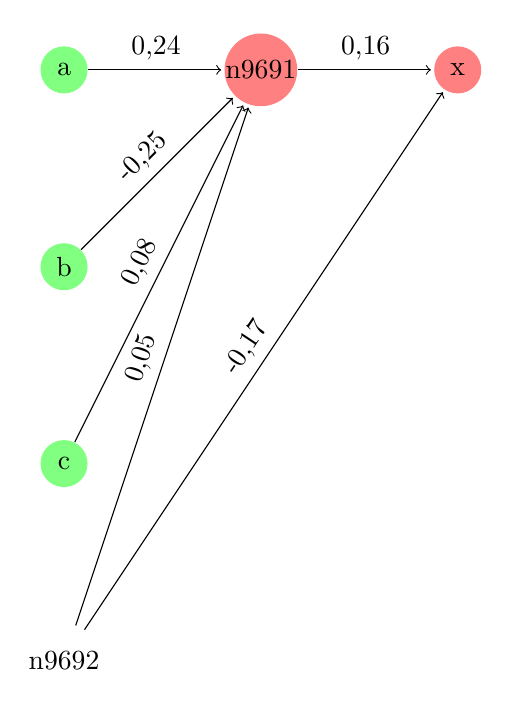
\begin{tikzpicture}[shorten >=1pt,->,draw=black!,node distance=2.5cm]
\tikzstyle{neuron}=[circle,fill=black!25,minimum size=17pt,inner sep=0pt]
\tikzstyle{constant}=[neuron, fill=white!50];
\tikzstyle{sigmoid}=[neuron, fill=red!50];
\tikzstyle{identity}=[neuron, fill=green!50];
\node [identity] (a) {a};
\node [identity,below of=a] (b) {b};
\node [identity,below of=b] (c) {c};
\node [constant,below of=c] (n9692) {n9692};
\node [sigmoid,right of=a] (n9691) {n9691};
\node [sigmoid,right of=n9691] (x) {x};
\path[every node/.style={sloped,anchor=south,auto=false}]
(n9692) edge node {0,05} (n9691)
(n9692) edge node {-0,17} (x)
(n9691) edge node {0,16} (x)
(a) edge node {0,24} (n9691)
(c) edge node {0,08} (n9691)
(b) edge node {-0,25} (n9691)
;\end{tikzpicture}
\end{document}